\documentclass{article}

\usepackage[francais]{babel}
\usepackage{graphicx}
\usepackage{amsmath}
\usepackage{amssymb}
\usepackage{gensymb}
\usepackage{listings}



\begin{document}

\title{Documentation de la suite logicielle GBMProject3A}
\author{Guillaume Gibert}
\maketitle

%%%SECTION%%%%%%%%%%%%
\section{Introduction}
Ce document décrit les différents éléments de la suite logicielle GBMProject3A.

	\subsection{Côté PC}
Le code fourni est écrit en C++ avec comme unique dépendance l'API Qt.
Il se compose d'un ensemble de classes qui permettent:
\begin{itemize}
	\item de communiquer avec un système Arduino que ce soit en réception ou en émission;
	\item de traiter des signaux (filtrage, FFT);
	\item d'afficher des signaux;
	\item de faire des requêtes sur une base de données MySQL.
\end{itemize}

	\subsection{Côté Arduino}
Un code de test est fourni qui permet d'envoyer sous forme de chaîne de caractères standardisée les valeurs lues sur les 5 canaux analogiques de la carte Arduino.
 Une fonction de lecture d'évènements est également mise en place pour lire, en parallèle, les données sur le port série provenant du PC.


Une série d'exemples permet d'implémenter chaque fonctionnalité. Ils vont être décrit dans la suite du document.

%%%SECTION%%%%%%%%%%%%
\section{Installation}

	\subsection{Qt}
Pour utiliser le code fourni dans ce projet, il faut installer l'API Qt.
Pour ce faire, il faut:
\begin{itemize}
	\item aller sur le site de Qt: https://www.qt.io/
	\item télécharger l'installateur pour la version Open Source (Onglet "Download. Try .Buy", puis "Go for Open Source", enfin "Download the Qt Online Installer");
	\item lancer l'installateur (vous devrez créer un compte Qt si vous n'en possédez pas) et choisir la version Open Source;
	\item choisir une version de Qt pour un compilateur donné (par exemple MinGW 64-bit)
	\item finaliser l'installation en suivant les instructions.
\end{itemize}

Une fois l'installation terminée, vous trouverez l'outil qtcreator.exe dans \textless QTDIR \textgreater/Tools/QtCreator/bin où \textless QTDIR \textgreater est le répertoire où vous avez choisi d'installer Qt.

	\subsection{Arduino}
Pour pouvoir utiliser la carte Arduino et charger vos programmes dans celle-ci, il faut installer l'IDE Arduino.
Pour ce faire, il faut:
\begin{itemize}
	\item aller sur le site d'Arduino: https://www.arduino.cc/
	\item télécharger l'installateur (Onglet "Software" puis "Downloads");
	\item lancer l'installateur;
	\item finaliser l'installation en suivant les instructions.
\end{itemize}

	\subsection{Github}
Pour récupérer le code de ce projet, deux options sont possibles:
\begin{itemize}
	\item Télécharger les sources
		\begin{itemize}
			\item aller sur le site: https://github.com/GuillaumeGibert/GBMProject3A;
			\item cliquer sud "Clone or download";
			\item cliquer "Download ZIP".
		\end{itemize}
	\item Cloner les sources
		\begin{itemize}
	 		\item aller sur le site: https://desktop.github.com/
			\item cliquer "Download for Windows";
			\item  installer Github Desktop;
			\item cloner le projet.
		\end{itemize}
\end{itemize}

	\subsection{GBMProject3A}
Il faut charger dans la carte Arduino le projet testArduino.ino qui se trouve dans \textless GBMProject3ADIR \textgreater/testArduino où \textless GBMProject3ADIR \textgreater/ est le répertoire où vous avez téléchargé les sources du projet.
Un programme Arduino est composé de 2 fonctions minimum:
\begin{itemize}
	\item une fonction setup() dans laquelle les variables sont initialisées qui est appelée une seule fois au début du programme;
	\item une fonction loop() qui est appelée réguliérement dès qu'elle est terminée.
\end{itemize}


Il faut ouvrir le fichier GBMProject3A.pro à l'aide du logiciel qtcreator.exe. 
Il faut ensuite éditer le fichier GBMProject3A.pro et changer la dernière ligne src/ex8.cpp par l'exemple que vous voulez lancer (choix possibles entre ex1, ex2, ex3, ex4, ex5, ex6, ex7 et ex8).
Pour créer votre propre programme, il vous suffit de créer un fichier main.cpp (par exemple) qui doit contenir une fonction main et d'éditer le fichier GBMProject3A.pro et changer la dernière ligne par src/main.cpp. 

%%%SECTION%%%%%%%%%%%%
\section{Code Arduino}
	\subsection{Variables globales}
Le code Arduino est composé de variables globales:
\begin{itemize}
	\item \textunderscore nbPinIn: nombre de pins analogiques connectés;
	\item \textunderscore portBaud: taux de transfert sur le port série;
	\item \textunderscore fps: fréquence de rappel de la fonction loop().
\end{itemize}

	\subsection{setup()}
La fonction setup() initalise le port série avec le taux de transfert spécifié dans la variable \textunderscore portBaud.

	\subsection{loop()}
La fonction loop() lit les valeurs sur les ports analogiques de la carte grâce à la commande analogRead(int). 
Elle crée une chaîne de caractères de la forme :  \begin{verbatim}Sensor:|<input1>|<input2>|<input3>|<input4>|<input5>|\n \end{verbatim}
Puis elle envoie cette chaîne de caractère sur le port série grâce à la fonction Serial.println(String).

	\subsection{serialEvent()}
La fonction serialEvent() est lancée entre deux appels à la fonction loop() si des données sont reçues sur le port série. 
Cela permet de récupérer sur la carte Arduino des informations en provenance du PC.


%%%SECTION%%%%%%%%%%%%
\section{Exemple 1: Récupérer des données depuis un Arduino (liaison filaire)}

Côté PC, deux objets sont instantiés (voir Figure~\ref{ex1}). Un objet de type SerialPortManager récupère les données envoyées par l'Arduino sur le port série. 
Il envoie ensuite, via un signal/slot Qt, les données vers un objet de type Spy qui les affiche à l'écran.

\begin{figure}
 \centering
    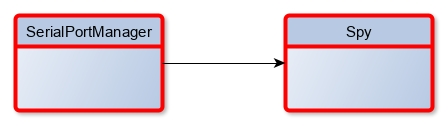
\includegraphics[width=10cm]{images/GBMProject3A_ex1.jpg}
    \caption{Les données de l'Arduino sont captées par l'objet SerialPortManager qui les envoie à l'objet Spy.}
    \label{ex1}
\end{figure}

%%%SECTION%%%%%%%%%%%%
%\begin{figure}
% \centering
%    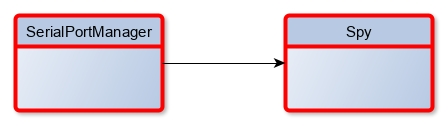
\includegraphics[width=10cm]{images/GBMProject3A_ex2.jpg}
%    \caption{Les données de l'Arduino sont captées par l'objet SerialPortManager qui les envoie à l'objet Spy.}
%    \label{ex2}
%\end{figure}

\section{Exemple 2: Récupérer des données depuis un Arduino (liaison Bluetooth)}

Cet exemple est similaire au précédent (cf. Figure~\ref{ex1}). La seule différence réside dans le type de connexion entre l'Arduino et le PC. 
Dans l'exemple précédent, L'Arduino était connecté avec un cable USB au PC alors que dans cet exemple, il est connecté en Bluetooth via un module HC-05 par exemple.

%%%SECTION%%%%%%%%%%%%
\section{Exemple 3: Récupérer des données depuis un générateur de signaux}

%%%SECTION%%%%%%%%%%%%
\section{Exemple 4: Afficher des signaux temporels}

%%%SECTION%%%%%%%%%%%%
\section{Exemple 5: Filtrer des signaux temporels}


%%%SECTION%%%%%%%%%%%%
\section{Exemple 6: Calculer une transformée de Fourier rapide (FFT)}


%%%SECTION%%%%%%%%%%%%
\section{Exemple 7:  Envoyer une chaîne de caractères à l'Arduino}

%%%SECTION%%%%%%%%%%%%
\section{Exemple 8:  Gérer une base de données "patient" depuis une interface graphique}

Il faut installer wamp. Attention il faut installer la même version que le compilateur de Qt (soit 32, soit 64bits).
Une fois installé, il faut compiler le plugin mysql qui n'est pas présent par défaut dans Qt. 
Il faut ouvrir une invite de commande, puis taper:
\begin{lstlisting}
cd %QTDIR%\qtbase\src\plugins\sqldrivers
qmake -- MYSQL_INCDIR="<WAMP_DIR>\bin\mysql\mysql5.7.28/include" 
MYSQL_LIBDIR="<WAMP_DIR>\bin\mysql\mysql5.7.28/lib"
nmake sub-mysql
nmake install
\end{lstlisting}
Si vous n'utilisez pas le compilateur de Visual Studio, il faudra remplacer nmake par mingw32-make


\end{document}